\begin{appendices}

\chapter{Implementazione}

Qui viene fatta una panoramica del codice delle classi e delle procedure essenziali alla realizzazione del progetto.
\newline

Il linguaggio utilizzato è Python 3.7 con il supporto delle librerie \\tensorflow e keras per la creazione e gestione delle reti neurali. Il client utilizzato per l'interazione col server di gioco è SnakeOil\cite{snakeoilWebsite}.

\clearpage

\section{Classe replayBuffer}

\inputminted[
frame=lines,
framesep=2mm,
fontsize=\footnotesize,
linenos
]{python}{Codes/replayBuffer.py}

Questa è la classe che implementa l'experience replay.
\newline

La classe definisce due metodi: uno per salvare una transizione in memoria e un altro per prelevare un batch di transizioni dalla memoria.

\clearpage

\section{Classe Critic}%\label{app:critic}

\inputminted[
frame=lines,
framesep=2mm,
fontsize=\footnotesize,
linenos
]{python}{Codes/critic.py}

La classe Critic racchiude tutti i metodi e le strutture dati per creare, usare e salvare la rete Critic.
\newline

Il cuore della classe è la funzione \textbf{\texttt{create\_critic}}. Essa riceve in ingresso il numero di neuroni del primo e del secondo livello denso nascosto e il learning rate. Nelle \textit{righe 21-23} si crea la parte della rete che prende in input lo stato \textit{s}, mentre nelle \textit{righe 25-26} si osserva la creazione della porzione della rete che lavora con l'azione \textit{a}.
\newline

Nella \textit{riga 28} vengono sommati i risultati intermedi di stato e azione e nella \textit{riga 29-30} si produce il risultato finale: il Q-value.

\clearpage

\section{Classe Actor}%\label{app:actor}

\inputminted[
frame=lines,
framesep=2mm,
fontsize=\footnotesize,
linenos
]{python}{Codes/actor.py}

La classe Actor racchiude tutti i metodi e le strutture dati per creare, usare e salvare la rete Actor.
\newline

La funzione \textbf{\texttt{create\_actor}} crea la rete neurale a partire dalle dimensioni dei due livelli densi nascosti e del learning rate. Si osservi, nelle \textit{righe 26-28} la creazione dei tre neuroni in uscita, fatta ognuna usando una diversa funzione di attivazione contenuta nel file di configurazione del modello.

\clearpage

\section{Classe Rumore}

\subsection{Ornstein-Uhlenbeck modificato}%\label{app:OU}

\inputminted[
frame=lines,
framesep=2mm,
fontsize=\footnotesize,
linenos
]{python}{Codes/ou.py}

\clearpage

Questa classe implementa il primo dei rumori esplorativi utilizzati.
\newline

Questo rumore è una variazione dell'\textit{Ornstein-Uhlenbeck} in quanto, come si vede nella \textit{riga 15}, nel 10\% dei casi viene prodotto un rumore gaussiano con media \textbf{\texttt{MU\textsubscript{2}}} e std \textbf{\texttt{STD\textsubscript{2}}} mentre nel 90\% dei casi viene prodotto un rumore in base al processo stocastico di Ornstein-Uhlenbeck.
\newline

Questo serve a fare in modo che l'agente sia sollecitato con due stimoli molto diversi fra loro in misure diverse. Nove volte su dieci si stimola l'agente ad andare molto veloce attraverso un rumore additivo con media alta sull'accelerazione e nulla sulla frenata e, una volta su dieci, invece, lo si stimola a frenare attraverso un rumore con una media nettamente inferiore sull'accelerazione e alta sulla frenata.
\newline


\clearpage


\subsection{Gaussian Noise}%\label{app:GN}

\inputminted[
frame=lines,
framesep=2mm,
fontsize=\footnotesize,
linenos
]{python}{Codes/gn.py}

Questo rumore è una variazione dell'\textit{$\epsilon$-greedy Gaussian Noise} in quanto, come si vede nella \textit{riga 18}, nel 90\% dei casi viene prodotto un rumore gaussiano con media \textbf{\texttt{MU\textsubscript{1}}} e std \textbf{\texttt{STD\textsubscript{1}}} mentre nel 10\% dei casi uno con media \textbf{\texttt{MU\textsubscript{2}}} e std \textbf{\texttt{STD\textsubscript{2}}}.
\newline

Questo serve a fare in modo che l'agente sia sollecitato con due stimoli molto diversi fra loro in misure diverse. Nove volte su dieci si stimola l'agente ad andare molto veloce attraverso un rumore additivo con media alta sull'accelerazione e nulla sulla frenata e, una volta su dieci, invece, lo si stimola a frenare attraverso un rumore con una media nettamente inferiore sull'accelerazione e alta sulla frenata.
\newline

La probabilità $\epsilon$ viene fatta decadere linearmente in un numero di passi pari a \textbf{\texttt{decay\_time}}.

\clearpage

\subsection{Time Variant Noise}%\label{app:TVNoise}
\inputminted[
frame=lines,
framesep=2mm,
fontsize=\footnotesize,
linenos
]{python}{Codes/tvnoise.py}
\clearpage

Questo classe implementa il TVNoise, un rumore gaussiano con media e std variabile nel tempo.
La classe restituisce un rumore gaussiano con media \textbf{\texttt{MU\textsubscript{1}}} e std \textbf{\texttt{STD\textsubscript{1}}} per i primi \textbf{\texttt{self.time\_step1}} passi.
\newline

Successivamente tende linearmente ad un rumore con distribuzione gaussiana con media \textbf{\texttt{MU\textsubscript{2}}} e std \textbf{\texttt{STD\textsubscript{2}}} in un numero di passi pari a \\\textbf{\texttt{(self.time\_step2 - self.time\_step1)}}.
\newline

Infine, sempre linearmente, tende ad avere media \textbf{\texttt{MU\textsubscript{3}}} e std \textbf{\texttt{STD\textsubscript{3}}} in \textbf{\texttt{(self.time\_step3 - self.time\_step2)}} passi. Nel progetto di tesi questo terzo passaggio viene sfruttato per far decadere a zero linearmente il rumore gaussiano aggiunto.
\newline

Nella fig.\ref{fig:tv_noise_media} viene mostrato un esempio di possibile andamento della media del rumore gaussiano. Lo stesso ragionamento si applica alla std.

\begin{figure}[hb]
    \center
    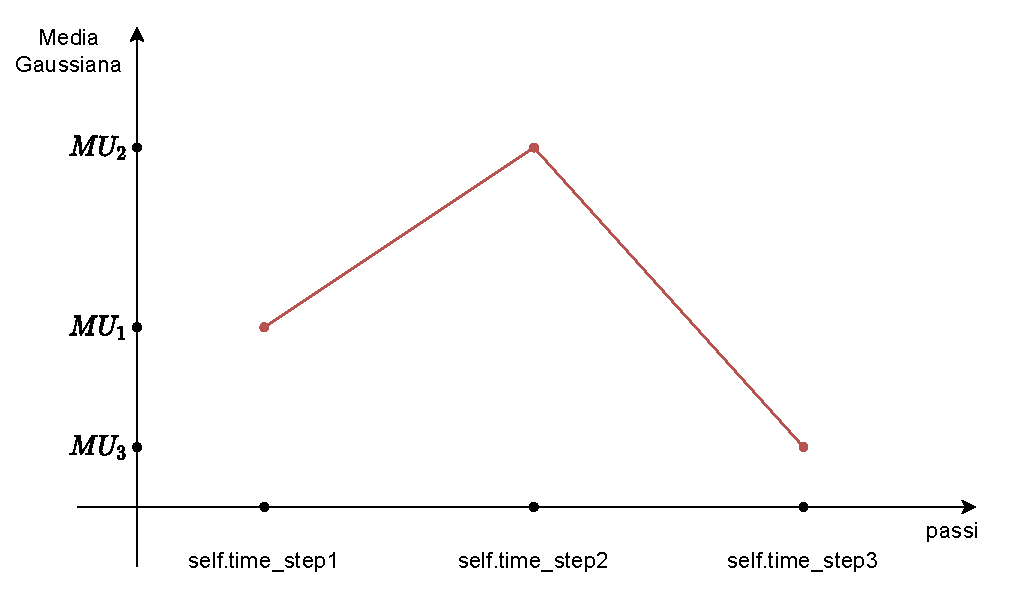
\includegraphics[width = 5in]{Figures/Appendix/tvnoise_media.drawio.pdf}
    \caption{Andamento della media Gaussiana}
    \label{fig:tv_noise_media}
\end{figure}

\clearpage

\section{Funzione train}

\inputminted[
frame=lines,
framesep=2mm,
fontsize=\footnotesize,
linenos
]{python}{Codes/train.py}

\clearpage

La funzione \textbf{\texttt{train}} è il cuore dell'algoritmo di apprendimento. In questa funzione vengono campionate la transizioni dall'experience replay, aggiornati i parametri delle reti Actor e Critic secondo i gradienti e, infine, aggiornate le reti target.
\newline

Nelle \textit{righe 16-28} vengono aggiornati i parametri della rete Critic. In particolare alla \textit{riga 23} viene calcolata la loss di eq.\ref{criticlossddpg} e alle \textit{righe 25-26} ne si calcola il gradiente rispetto ai parametri della rete.
\newline

Nelle \textit{righe 30-39} vengono aggiornati i parametri della rete Actor. Si noti come alla \textit{riga 32} viene invertito il segno ai valori prodotti dal Critic: questo serve poiché l'ottimizzatore utilizzato effettua una discesa del gradiente, quindi invertendo il segno ai valori si effettuerà una salita lungo il gradiente, come imposto dalla eq.\ref{gradactorddpg}. Nella \textit{righe 36-37} viene effettivamente calcolato il gradiente della $Q$ rispetto ai parametri della rete Actor.


\clearpage

\section{Funzione update\_target}

\inputminted[
frame=lines,
framesep=2mm,
fontsize=\footnotesize,
linenos
]{python}{Codes/update_target.py}

La funzione che effettua il soft update delle reti target in ottemperanza alle eq.\ref{ddpgsoftupdate_eq}. Lo \textbf{\texttt{sm\_fact}}, ovvero smooth factor, identifica la $\tau$.

\clearpage

\section{Funzione reward}\label{app:reward}

\subsection{Reward standard}\label{app:reward_standard}

\inputminted[
frame=lines,
framesep=2mm,
fontsize=\footnotesize,
linenos
]{python}{Codes/reward_standard.py}

Codice della reward standard. Restituisce $-200$ se l'agente è fuori carreggiata oppure un numero reale calcolato nella \textit{riga 6}.

\subsection{Reward senza trackPos}\label{app:reward_notrackpos}

\inputminted[
frame=lines,
framesep=2mm,
fontsize=\footnotesize,
linenos
]{python}{Codes/reward_notrackpos.py}

L'unica differenza dalla reward standard è che nella \textit{riga 6} viene rimossa la penalizzazione rispetto alla distanza dal centro della carreggiata. Viene ovviamente mantenuto il controllo di uscita da essa nelle \textit{righe 3-4}.

\subsection{Reward con angle}\label{app:reward_notrackpos_angle}

\inputminted[
frame=lines,
framesep=2mm,
fontsize=\footnotesize,
linenos
]{python}{Codes/reward_notrackpos_angle.py}

Questa reward sostituisce la penalizzazione rispetto alla distanza dal centro della carreggiata con una rispetto all'angolo della vettura rispetto all'asse della carreggiata.

\clearpage


	
\end{appendices}